\documentclass[8pt,a4paper,landscape]{article}
\usepackage[utf8]{inputenc}
\usepackage[english]{babel}
\usepackage{amsmath}
\usepackage{amsfonts}
\usepackage{amsthm}
\usepackage{amssymb}
\usepackage{graphicx}
\usepackage{float}
\usepackage[left=0.75cm,right=0.75cm,top=0.75cm,bottom=1.4cm]{geometry}
\usepackage[skins]{tcolorbox}
\usepackage{multicol}
\usepackage{calrsfs}
\usepackage{xcolor}
\usepackage{csquotes}
\usepackage{mathtools}
\usepackage{hyperref}
\usepackage{enumitem}


\definecolor{DarkGreen}{RGB}{1,100,32}

\setlength{\columnseprule}{1pt}

% Redefine the 'definition' style to have italic text
\newtheoremstyle{definition}      % Name (must match the one you're overriding)
  {\topsep}                       % Space above
  {\topsep}                       % Space below
  {\normalfont}                      % Body font -> italic
  {}                              % Indent amount
  {\bfseries}                     % Theorem head font
  {.}                             % Punctuation after theorem head
  { }                             % Space after theorem head
  {}                              % Theorem head spec
\theoremstyle{definition}
\newtheorem{definition}{Def.}[section]

\newtheoremstyle{example}      % Name of style
  {\topsep}                           % Space above
  {\topsep}                           % Space below
  {\itshape}                       % Body font (non-italic)
  {}                                  % Indent amount
  {\bfseries}                         % Theorem head font
  {.}                                 % Punctuation after theorem head
  { }                                 % Space after theorem head
  {}                                  % Theorem head spec
\theoremstyle{example}
\newtheorem{example}{Ex.}[section]

% Custom theorem style: intuition
\newtheoremstyle{intuition}    % Name
  {\topsep}                       % Space above
  {\topsep}                       % Space below
  {\color{DarkGreen}\normalfont}                   % Body font -> upright
  {}                              % Indent amount
  {\color{black}\bfseries}    % Theorem head font
  {.}                             % Punctuation after theorem head
  { }                             % Space after theorem head
  {}                              % Theorem head spec
\theoremstyle{intuition}
\newtheorem*{intuition}{Int}

\theoremstyle{definition}
\newtheorem{proposition}{Prop}[section]

\DeclareMathAlphabet{\pazocal}{OMS}{zplm}{m}{n}
%\newcommand{\La}{\mathcal{L}}
\newcommand{\Lb}{\pazocal{L}}
%\newcommand{\Fa}{\mathcal{F}}
\newcommand{\Fb}{\pazocal{F}}
\newcommand{\Pb}{\pazocal{P}}

\newcommand{\mydef}[1]{\textcolor{magenta}{\textbf{#1}}}
\newcommand{\prob}[1]{\mathbb{P}\left[ #1 \right]}

\DeclarePairedDelimiter\abs{\lvert}{\rvert}%
\DeclarePairedDelimiter\norm{\lVert}{\rVert}%

\MakeOuterQuote{"}


\author{Marc-Olivier Jufer \\ \href{mailto:mjufer@ethz.ch}{mjufer@ethz.ch}}
\title{Cheatsheet Probability and Statistics}


\begin{document}
\begin{multicols}{3}
	\maketitle
	
	
	\section{Mathematical framework}
			\subsection{Probability space}
			
			
				%sample space, outcome, elementary experiment
				\begin{definition}
					The set $\Omega$ is called the \mydef{sample space}. An element $\omega \in \Omega$ is called an \mydef{outcome} or \mydef{elementary experiment}.
				\end{definition}
				\begin{example}
					Throw of a die : $\Omega = \{1,2,3,4,5,6\}$
				\end{example}
				
				
				% sigma-algebra
				\begin{definition} \label{dsa}
					A \mydef{sigma-algebra} is a subset $\Fb \subset \Pb (\Omega)$ satisfying the following properties :
					\begin{description}
						\item[P1.] $\Omega \in \Fb$
						\item[P2.] $A \in \Fb \Rightarrow A^c \in \Fb$ : \textcolor{DarkGreen}{If $A$ is an event, "not $A$" is also an event.}
						\item[P3.] $A_1, A_2, \ldots \in \Fb \Rightarrow \bigcup\limits_{i=1}^{\infty}A_i \in \Fb$ : \textcolor{DarkGreen}{if $A_1, A_2, \ldots$ are events, then "$A_1$ or $A_2$ or $\ldots$" is an event}
					\end{description}
				\end{definition}
				\begin{example}
					Examples of sigma-algebras for $\Omega = \{1,2,3,4,5,6\}$ :
					\begin{itemize}
						\item $\Fb = \{\emptyset, \{1,2,3,4,5,6\}\}$
						\item $\Fb = \Pb(\Omega)$
						\item $\Fb = \{\emptyset, \{1,2\}, \{3,4,5,6\}, \{1,2,3,4,5,6\}\}$
					\end{itemize}
					Non examples of sigma-algebras for $\Omega = \{1,2,3,4,5,6\}$ :
					\begin{itemize}
						\item $\Fb  = \{\{1,2,3,4,5,6\}\}$ : \textbf{P2} is not satisfied
						\item $\Fb = \{\emptyset, \{1,2,3\},\{4,5,6\},\{1\},\{2,3,4,5,6\},\Omega\}$ : \textbf{P3} is not satisfied
					\end{itemize}
				\end{example}
				
				
				% probability measure
				\begin{definition} \label{dpm}
					Let $\Omega$ a sample space and $\Fb$ a sigma-algebra. A \mydef{probability measure} on $(\Omega, \Fb)$ is a map
					$$
						\mathbb{P}: \Fb \to \left[0,1\right], \quad A \mapsto \mathbb{P}\left[A\right] 
					$$
					that satisfies the properties
					\begin{description} 
						\item[P1.] $\mathbb{P}[\Omega] = 1$
						\item[P2. (countable additivity)] $\mathbb{P}[A] = \sum_{i=1}^{\infty} \mathbb{P}[A_i]$ if $A = \bigcup_{i=1}^{\infty} A_i$ (disjoint union)
					\end{description}
				\end{definition}
				\begin{intuition}
					A probability measure is a map that associates to each event a number in $[0,1]$
				\end{intuition}
				\begin{example}
					For $\Omega = \{1,2,3,4,5,6\}$ and $\Fb = \Pb(\Omega)$, the mapping $\mathbb{P}: \Fb \to [0,1]$ defined by 
					$$
						\forall A \in \Fb \quad \mathbb{P}[A] = \frac{\abs{A}}{6}
					$$
					is a probability measure on $(\Omega, \Fb)$.
				\end{example}
				
				
				% probability space
				\begin{definition}
					Let $\Omega$ a sample space, $\Fb$ a sigma-algebra and $\mathbb{P}$ a probability measure. The triple $(\Omega, \Fb, \mathbb{P})$ is called a \mydef{probability space}.
				\end{definition}
				
				
				% summary mathematical framework
				\begin{intuition}
					To construct a probabilistic model, we give
					\begin{itemize}
						\item a sample space $\Omega$ : all the possible outcomes of the experiment
						\item a sigma-algebra $\Fb \subset \Pb(\Omega)$ : the set of events
						\item a probability measure $\mathbb{P}$ : gives a number in $[0,1]$ to every event
					\end{itemize}
				\end{intuition}
				
				
				% occurs
				\begin{definition}
					Let $\omega \in \Omega$ (a possible outcome). Let $A$ be an event. We say the event $A$ \mydef{occurs} (\mydef{does not occur}) (for $\omega$) if $\omega \in A$ ($\omega \notin A$).
				\end{definition}
				
				
				
			\subsection{Examples of probability spaces}
			
				\begin{definition}
					Let $\Omega$ be a finite sample space. The \mydef{Laplace model} on $\Omega$ is the triple $(\Omega,\Fb, \mathbb{P})$, where $\Fb = \Pb(\Omega)$ and $\mathbb{P}: \Fb \to \left[0,1\right]$ is defined by
						$$
							\forall A \in \Fb \quad P\left[ A \right] = \frac{\abs{A}}{\abs{\Omega}}
						$$
				\end{definition}
				
				
			\subsection{Properties of Events}
				
				\begin{proposition}
					(Consequences of definition \ref{dsa}). Let $\Fb$ be a sigma-algebra on $\Omega$. We have
					\begin{description} 
						\item[P4.]  $\emptyset \in \Fb$
						\item[P5.] $A_1, A_2, \ldots \in \Fb \Rightarrow \bigcap_{i=1}^{\infty}A_i \in \Fb$
						\item[P6.] $A,B \in \Fb \Rightarrow A \cup B \in \Fb$
						\item[P7.] $A,B \in \Fb \Rightarrow A \cap B \in \Fb$
					\end{description}
				\end{proposition}
				
				\begin{figure}[H]
					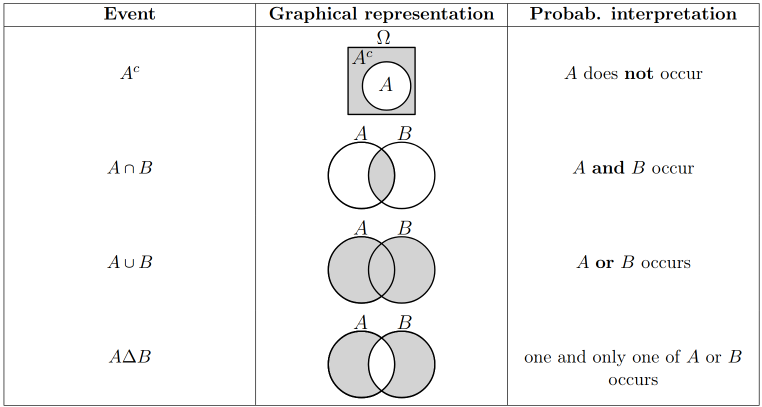
\includegraphics[width=\linewidth]{set-operations-representation.png}
					\caption{Representation of set operations}
				\end{figure}
				
%				Other set relations probabilistic interpretation :
%				\begin{itemize}
%					\item $A \subset B$ : If $A$ occurs, then $B$ occurs
%					\item $A \cap B = \emptyset$ : $A$ and $B$ cannot occur at the same time
%					\item $\Omega = A_1 \cup A_2 \cup A_3$ with $A_1,A_2,A_3$ pairwise disjoint : for each outcome $\omega$, one and only on of the events $A_1, A_2, A_3$ is satisfied.
%				\end{itemize}
				
				\begin{figure}[H]
					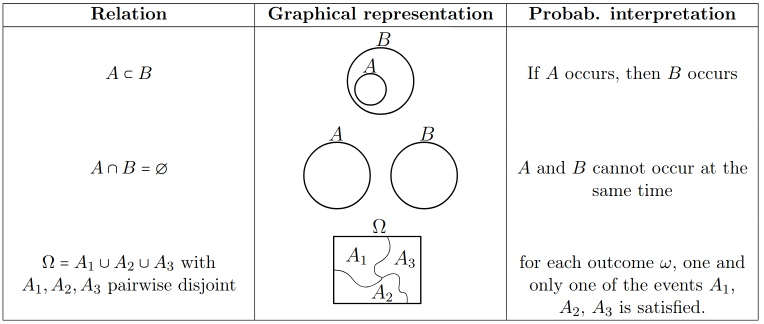
\includegraphics[width=\linewidth]{set-relations-representation.png}
					\caption{Representation of set relations}
				\end{figure}
				
				
			\subsection{Properties of probability measures}
			
				\begin{proposition}	
					(Consequences of definition \ref{dpm}). Let $\mathbb{P}$ be a probability measure on $(\Omega, \Fb)$.
					\begin{description}
						\item[P3.] We have $\mathbb{P}\left[\emptyset\right] = 0$
						\item[P4.] (\mydef{additivity}) Let $k \geq 1$, let $A_1, \ldots , A_k$ be $k$ pairwise disjoint events, then 
							$$
								\mathbb{P}\left[A_1 \cup \ldots \cup A_k \right] = \prob{A_1} + \ldots + \mathbb{P}\left[ A_k \right]
							$$
						\item[P5.] Let $A$ be an event, then
							$$
								\prob{A^c} = 1 - \prob{A}
							$$
						\item[P6.] If $A$ and $B$ are two events (not necessarily disjoint), then 
							$$
								\prob{A \cup B} = \prob{A} + \prob{B} - \prob{A \ cap B}
							$$
					\end{description}
				\end{proposition}
				
				\begin{proposition}
					(\mydef{Monotonicity}). Let $A, B \in \Fb$, then
					$$
						A \subset B \Rightarrow \prob{A} \leq \prob{B}
					$$
				\end{proposition}
				
				\begin{proposition}
					(\mydef{Union bound}).Let $A_1, A_2, \ldots$ be a sequence of events (not necessarily disjoint), then we have
					$$
						\prob{\bigcup\limits_{i=1}^{\infty} A_i} \leq \sum_{i=1}^{\infty}\prob{A_i}
					$$
					Union bound also applies to a finite collection of events.
				\end{proposition}
				
				\begin{proposition}
					Let $(A_n)$ be an increasing sequence of events (i.e. $\forall n \ A_n \subset A_{n+1}$). Then
					\begin{center}
						$\lim_{n \rightarrow \infty} \prob{A_n} = \prob{\bigcup\limits_{n=1}{\infty} A_n}$. \mydef{increasing limit}
					\end{center}
					Let $(B_n)$ be a decreasing sequence of events (i.e. $\forall n \ B_n \supset B_{n+1}$). Then
					\begin{center}
						$\lim_{n \rightarrow \infty} \prob{B_n} = \prob{\bigcap\limits_{n=1}{\infty} B_n}$. \mydef{decreasing limit}
					\end{center}
				\end{proposition}
				
				
			\subsection{Conditional probabilities}
			
				% Conditional probabilitiy
				\begin{definition}
					Let $(\Omega, \Fb, \mathbb{P})$ be some probability space. Let $A, B$ be two events with $\prob{B} > 0$. The \mydef{conditional probability of} $A$ \mydef{given} $B$ is defined by
					$$
						\prob{A \lvert B} = \frac{A \cap B}{B}
					$$
				\end{definition}
				
				\begin{example}
					We consider the probability space $(\Omega, \Fb, \mathbb{P})$ corresponding to the throw of one die. Let $A = \{1,2,3\}$ and $B = \{2,4,6\}$. Then
					$$
						\prob{A \lvert B} = \frac{\prob{A \cap B}}{\prob{B}} = \frac{\frac{1}{6}}{\frac{1}{2}} = \frac{1}{3}
					$$
				\end{example}
				
				\begin{proposition}
					Let $(\Omega, \Fb, \mathbb{P})$ be some probability space. Let $B$ be an event with positive probability. Then $\prob{\ . \ \lvert B}$ is a probability measure on $\Omega$.
				\end{proposition}
				
				% Total probability
				\begin{proposition}
					(\mydef{Formula of total probability}). Let $B_1, \ldots, B_n$ be a partition\footnote{i.e. $\Omega = B_1 \cup \ldots \cup B_n$ and the events are pairwise disjoint.} of the sample space $\Omega$ with $\prob{B_i} > 0$ for every $i \leq i \leq n$. Then one has
					$$
						\forall A \in \Fb \quad \prob{A} = \sum_{i=1}^n \prob{A \lvert B_i} \prob{B_i}
					$$
				\end{proposition}
				
				% Bayes formula
				\begin{proposition}
					(\mydef{Bayes formula}). Let $B_1, \ldots, B_n \in \Fb$ be a partition of $\Omega$ with $\prob{B_i} > 0 \ \forall i$. For every event $A$ with $\prob{A} > 0$ we have 
					$$
						\forall i = 1, \ldots, n \quad \prob{B_i \lvert A} = \frac{\prob{A \vert B_i} \prob{B_i}}{\sum_{j=1}^n \prob{A \lvert B_j} \prob{B_j}}
					$$
				\end{proposition}
				
				\begin{example}
					Test to detect a disease which concerns about $1/10000$ of the population. The test gives the right answer $99\%$ of the time. If a patient has a positive test, what is the probability that he is actually sick ?\\
					We modeled the situation as $\Omega = \{0,1\} \times \{0,1\}$. $\Fb = \Pb(\Omega)$ and an outcome is $\omega = (\omega_1, \omega_2)$, where $\omega_1$ is $1$ if the patient is sick and $\omega_2$ is $1$ if the test is positive. Let $S = \{(1,0), (1,1)\}$ be the event that the patient is sick and $T = \{(0,1),(1,1)\}$ the event that the test is positive.\\
					From the hypotheses, we have
					$$
						\prob{S} = \frac{1}{10000}, \quad \prob{T \lvert S} = \frac{99}{100}, \quad \prob{T \lvert S^c} = \frac{1}{100}
					$$
					By applying the Bayes formula to the partition $\Omega = S \cup S^c$, we obtain
					$$
						\prob{S \lvert T} = \frac{\prob{T \lvert S} \prob{S}}{\prob{T \lvert S} \prob{S} + \prob{T \lvert S^c} \prob{S^c}} \simeq 0.0098
					$$
				\end{example}
				
				
			\subsection{Independence}
			
				% Independence of events
				\begin{definition}
					Let $(\Omega, \Fb, \mathbb{P})$ be a probability space. Two events $A$ and $B$ are said to be \mydef{independent} if 
					$$
						\prob{A \cap B} = \prob{A} \prob{B}
					$$
					$A$ is independent of $B$ iff $A$ is independent of $B^c$. \\
					If $\prob{A} \in \{0,1\}$, then $A$ is independent of every event. \\
					If $A$ is independent with itself (i.e. $\prob{A \cap A} = \prob{A}^2$), then $\prob{A} \in \{0, 1\}$.
				\end{definition}
				
				\begin{proposition}
					Let $A, B \in \Fb$ be two events with $\prob{A}, \prob{B} > 0$. Then the following are equivalent :
					\begin{enumerate}[label=\roman*.]
						\item $\prob{A \cap B} = \prob{A} \prob{B}$ : \textcolor{DarkGreen}{A and B are independent}
						\item $\prob{A \lvert B} = \prob{A}$ : \textcolor{DarkGreen}{the occurrence of B has no influence on A}
						\item $\prob{B \lvert A} = \prob{B}$ : \textcolor{DarkGreen}{the occurrence of A has no influence on B}
					\end{enumerate} 
				\end{proposition}
				
				% Independence of collection of events
				\begin{definition}
					Let $I$ be an arbitrary set of indices. A collection of events $(A_i)_{i \in I}$ is said to be \mydef{independent} if 
					$$
						\forall J \subset I finite \quad \prob{\bigcap\limits_{j \in J} A_j} = \prod_{j \in J} \prob{A_j}
					$$
				\end{definition}
				
				\begin{intuition}
					Three events $A$, $B$ and $C$ are independent if the following 4 equations are satisfied :
						$$\prob{A \cap B} = \prob{A} \prob{B} $$
						$$\prob{A \cap C} = \prob{A} \prob{C} $$
						$$\prob{B \cap C} = \prob{B} \prob{C} $$
						$$\prob{A \cap B \cap C} = \prob{A}\prob{B}\prob{C}$$
				\end{intuition}


	\newpage
	\section{Random variables and distribution functions}
			\subsection{Abstract definition}
			
				% Random variable
				\begin{definition}
					Let $(\Omega, \Fb, \mathbb{P})$ be a probability space. A \mydef{random variable} (r.v.) is a map $X : \Omega \to \mathbb{R}$ s.t.
					$$						
						\forall a \in \mathbb{R} \quad \{\omega \in \Omega : X(\omega) \leq a\} \in \Fb
					$$
				\end{definition}
				
				
				
	
	
\end{multicols}	
\end{document}